\section{Introduction}

This thesis considers applying learning classifier systems (LCS's) to the prediction of time series data.
A time series as used here is a sequence of data successively measured through time.
Time series analysis encompasses many methods that attempt to understand such time series, aimed at either understanding the underlying theory present in the data points or to make real-world predictions.
Time series prediction is the use of a model to predict future events based on known past events: to predict future data points before they are measured.
One standard example is the opening price of a share of stock based on its past performance.

%\vspace*{-\baselineskip}    %You need to place this before a 
                            %subsection if it immediately follows
                            %section.
\subsection{Motivation}
No LCS to date has been designed for time series data but instead they were generally limited to Markov systems lacking any memory, which we viewed as a major limitation of LCS's.
LCS's are designed specifically with the concept of evolving an effective rule set for a specified problem, which is specifically the sort of capability that would be desirable for time series analysis and prediction: generating useful rule sets.

An LCS is an evolutionary algorithm that operates on a population comprised of rules referred to as the rule set: this rule set is used to attempt to classify a situation.
The first LCS was created by Holland \cite{HollandLCS} shortly after he created genetic algorithms (GA's) \cite{HollandGA}, one of the classical types of evolutionary algorithms.
Holland's first LCS originally used a GA as the evolutionary device.
Our system as described here also uses a GA for evolution, although it has been modified from the original form.

Holland's original LCS was quite complicated and failed to produce quality results for most real-world problems.
Because of this, the study of LCS's was somewhat inactive until Wilson introduced ZCS \cite{WilsonZCS}, a re-imagining of Holland's original LCS distilled to its most basic elements.
Wilson's ZCS was capable of producing acceptable results on certain problems and was simple enough to easily understand, reinvigorating LCS research.

A few years after introducing ZCS, Wilson modified it introducing XCS \cite{Wilson1995XCS}, which is currently one of the best performing and most popular LCS types.
Wilson's XCS was based on ZCS but with several important modifications mostly aimed at improving the accuracy of the rules produced and also for a more full coverage of the problem space by the rules.
A significant portion of the LCS's being worked on today are modifications or enhancements of Wilson's XCS.

One such enhancement of XCS is known as XCSR \cite{WilsonXCSR}, which was also developed by Wilson.
XCSR improves upon XCS by allowing it to operate with real-valued ranges for input instead of on the traditional ternary alphabet so common to LCS's, consisting of \emph{true}, \emph{false}, and a covering symbol (usually represented as $\#$ or $*$).

\subsection{Background}
The system presented here is derived from Wilson's XCSR, which is an extension of Wilson's XCS, which in turn was derived from Wilson's ZCS.
ZCS, XCS, XCSR, and this system are all learning classifier systems (LCS's), a crossover of the fields of evolutionary computation (EC) and reinforcement learning (RL), both of which are quite large fields on their own.
We will describe in this section the previous works this system was built upon.

\subsection{Reinforcement Learning}
Reinforcement learning \cite{SuttonBarto:1998a} is the process of learning how to map situations to actions to maximize a numerical reward.
The learning system is not told which actions to take, as in most forms of machine learning, but instead must discover which actions yield the most reward by exploration.
In the most interesting and challenging cases, actions may affect not only the immediate reward but also the next situation and, through that, all subsequent rewards.  
The two primary distinguishing characteristics of reinforcement learning are:
\begin{enumerate}
\item trial-and-error search and
\item delayed reward.
\end{enumerate}
Reinforcement learning is defined not by characterizing learning methods, but by characterizing a learning problem.
We consider any method that is well suited to solving that problem to be a reinforcement learning method.
The idea is to capture the most important aspects of the problem facing the learning agent interacting with its environment to achieve its goal.
Such an agent must be able to:
\begin{enumerate}
\item perceive the state of the environment,
\item act on the environment, and
\item have a goal or goals relating to the state of the environment.
\end{enumerate}
Tersely put: \textit{sensation}, \textit{action}, and \textit{goal}.

\subsubsection{Exploration versus Exploitation}
A primary challenge is the trade-off between exploration and exploitation.  A reinforcement learning agent will prefer actions that it has tried in the past and found to be effective in producing reward in order to reliably obtain more reward.  But to discover such actions, it has to try actions that it has not selected before.  The agent has to \textit{exploit} existing knowledge to obtain reward, but it also must \textit{explore} to make better action selections in the future.  Neither exploration nor exploitation can be pursued exclusively without failure.  The agent must try a variety of actions and progressively favor those that appear to be best.  On a stochastic task, each action must be tried many times to gain a reliable estimate of its expected reward.

\subsubsection{The Whole Problem}
Reinforcement learning explicitly considers the whole problem of a goal-directed agent interacting with an uncertain environment,  starting with a complete, interactive, goal-seeking agent, instead of considering subproblems without addressing how they might fit into a larger picture.  All reinforcement learning agents have explicit goals, can sense aspects of their environments, and can choose actions to influence their environments.  From the beginning, the agent operates with significant uncertainty about its environment.  For learning research to make progress, important subproblems have to be isolated and studied, but they should be subproblems that play clear roles in complete, interactive, goal-seeking agents, even if all the details of the complete agent cannot yet be filled in.


\subsection{Evolutionary Algorithms}
In artificial intelligence (AI), evolutionary algorithms (EA's) are a style of generic population-based meta-heuristic optimization algorithms whose processes are inspired by those of natural biological evolution.
The primary mechanisms employed in EA's to evolve a population of possible solutions towards an optimal one are:
\begin{enumerate}
\item parent selection based on fitness,
\item recombination,
\item mutation, and
\item and survivor selection based on fitness.
\end{enumerate}
Evolution serves as a powerful metaphor and demonstrates great creativity in both the natural world and in the world of computer science.

In normal biological evolution the environment that the population exists in exerts various pressures on the individuals in the population that determines the likelihood that any particular individual will manage to survive long enough to reproduce, and it is through this process that the fitness of an individual in the population must be determined: relative to its environment.
In an EA, the environment relates to the problem we wish to solve, the individuals in the population encode potential solutions to that problem, and their fitness is their quality as a solution to the problem.
By mimicking the methods of natural evolution in this manner we can often arrive at good solutions.
The basic evolutionary process is outlined in Algorithm~\ref{alg:evolution}.

\begin{algorithm}[H]
\caption{The evolutionary process.}
\begin{algorithmic}[1]
\label{alg:evolution}
\STATE
Initialize the population, either with randomly-generated or seeded candidate solutions or both.
\STATE
Evaluate the fitness of each member of the population.
\REPEAT
  \STATE
  Select members of the population to act as parents.
  This is typically related to the relative fitness of the parents in some way.
  \STATE
  Recombine the genetic material of the parents, producing offspring to be added to the population.
  \STATE
  Mutate some or all of the newly-created offspring.
  \STATE
  Evaluate the fitness of the offspring.
  \STATE
  Select survivors from the current population or a subset thereof, often only the newly-created offspring, to survive to the next generation.
\UNTIL{some specified termination condition is satisfied.}
\end{algorithmic}
\end{algorithm}


\subsubsection{Learning Classifier Systems}
A learning classifier system is a type of EA in which a description of a current situation is used in an attempt to map that description to some classification or action.
This is achieved through simulated evolutionary processes, where the population being evolved consists of various rules;
our entire population forms a rule set, and we apply concepts from Darwinism to our individual rules.
This is known in learning classifiers as the \emph{Michigan approach} \cite{EibenSmith}.
The other primary method employed, where each individual is an entire solution, and therefore a whole rule set, is known as the \emph{Pittsburgh approach}.
We use a modification of XCSR here, which uses the Michigan approach, and therefore so do we.

\subsubsection{ZCS}
\index{ZCS}
ZCS is a \emph{zeroth level classifier system} originally proposed in \cite{WilsonZCS}.
ZCS preserves most of the functionality of traditional LCS's, but it is a very simplified version, which aids in the understanding of the classifier and its actions.
This was a very useful contribution, because many of the problems with LCS's before then were their overly complex and detailed nature.
A good short summary of ZCS can be found in
\cite{EibenSmith}, and this summary is based primarily on that.
The basic structure of ZCS is graphically illustrated in Figure~\ref{fig:zcs}.

In ZCS there is no message list, a much-welcomed simplification of the traditional LCS.
This comes with a cost: there is no explicit method for transmitting information between cycles without the message list.
This makes the interface entirely dependent on the interface of the system with its environment, and thus assumes a Markov process.
This is most definitely an invalid assumption for real-world traded markets and for other time-series data.

\begin{figure}
\begin{center}
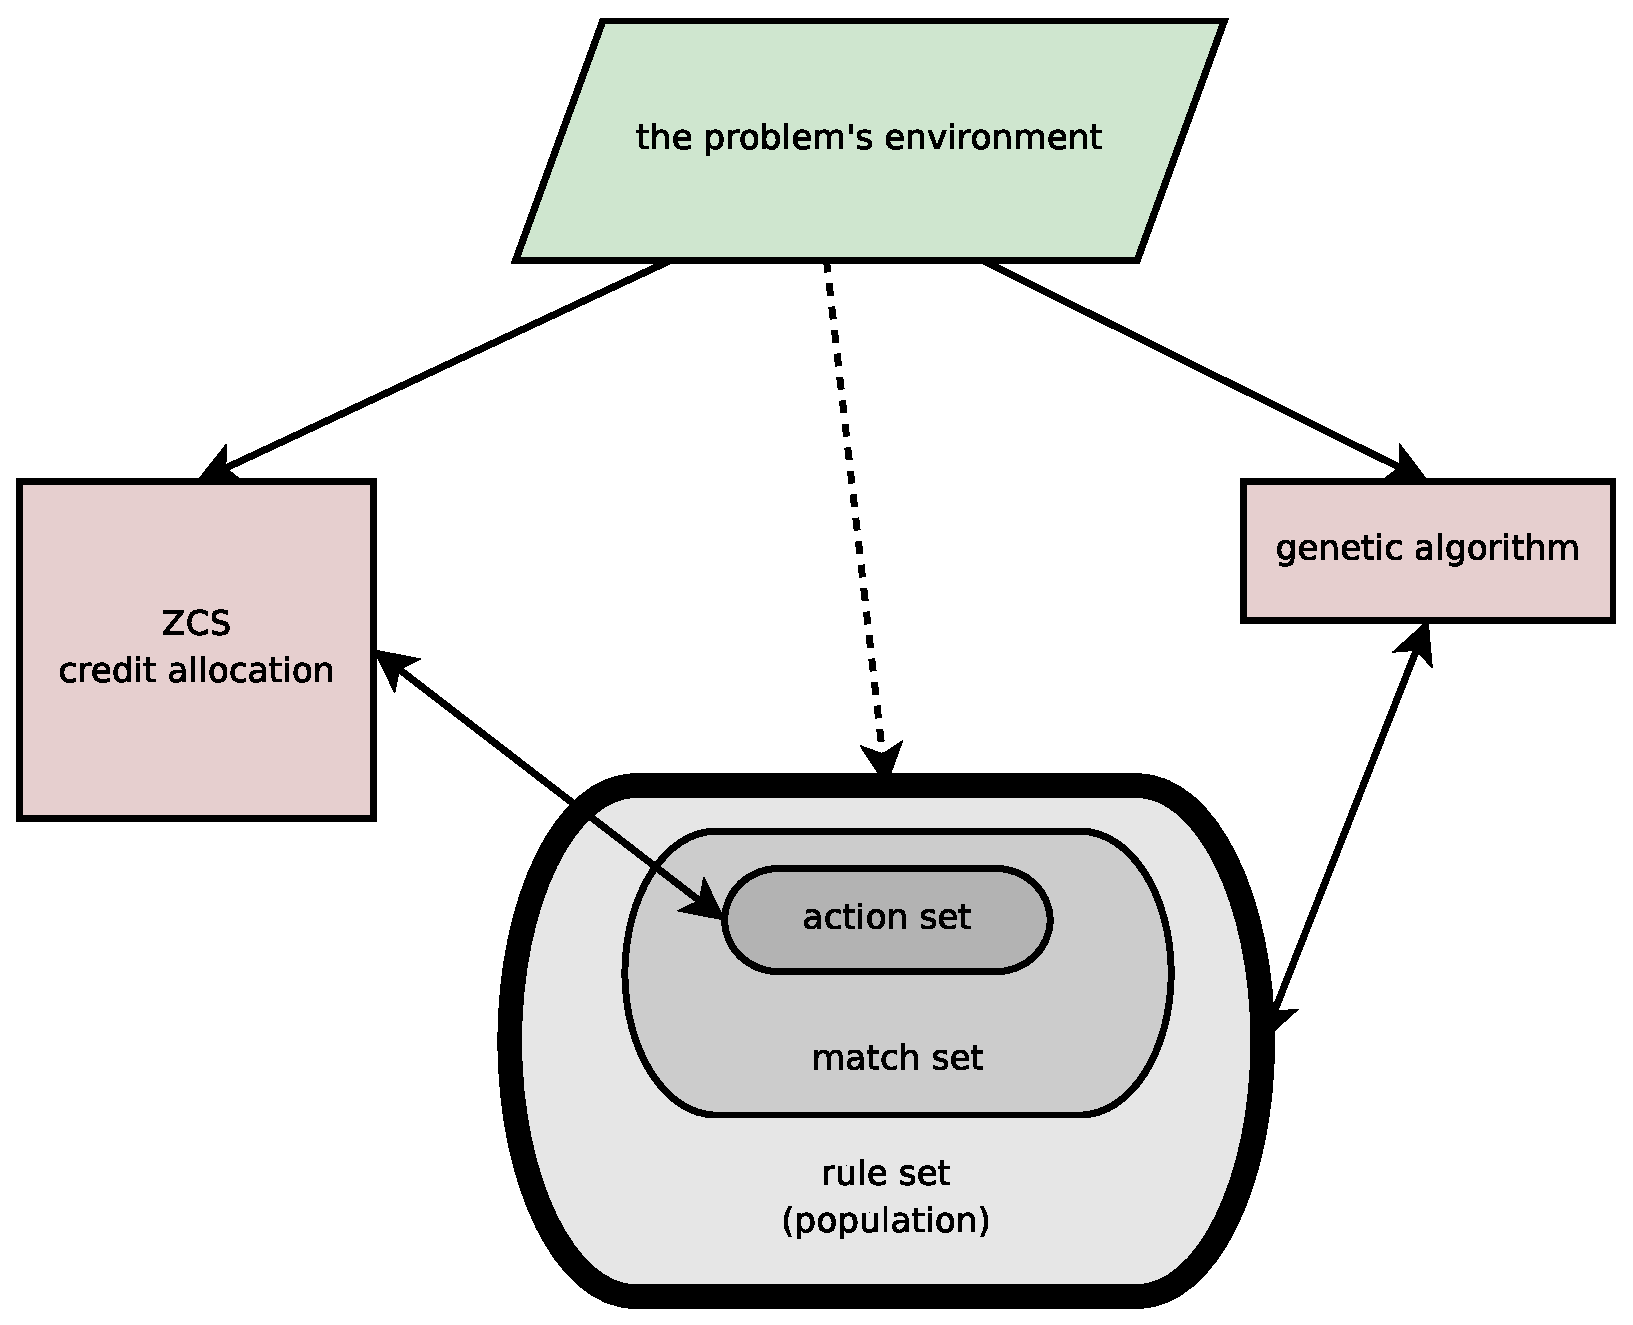
\includegraphics[width=4in]{zcs-basic-diagram.eps}
\caption{ZCS's basic structure}
\label{fig:zcs}
\end{center}
\end{figure}

Each rule $r$ is of the form $r = (c, a, s)$ where:
\begin{itemize}
\item
$c$ is the condition matched by the rule $r$ and is comprised of elements from some alphabet, typically $\{0, 1, \#\}$,
where \# is the matching symbol, matching both 0 and 1;
\item
$a$ is the action that the rule $r$ recommends;
\item
and $s$ is the real-valued strength measurement of the rule $r$, $s \in \mathbb{R}$, which determines how much of a vote rule $r$ has in selecting the action to pursue.
\end{itemize}

In each time cycle $t$ the match set $M_t$ is found, a subset of the population,
$M_t \subseteq P$,
with $P$ being the entire population of rules, the rule set.
\index{population}
\index{P@$P$|see{population}}
The members at time cycle $t$ of the match set $M_t$ can be divided into disjoint subsets based on the action they recommend.
With a finite set of possible actions
\begin{equation}
\mathpzc{A} = \{a_0, a_1, \ldots, a_{|\mathpzc{A}|}\}
\end{equation}
and $\mathpzc{A'} \subseteq \mathpzc{A}$ where
\begin{equation}
\mathpzc{A'} = \{a'_0, a'_1, \ldots, a'_{|\mathpzc{A'}|}\}
\end{equation}
comprises all of the actions represented in the match set $M_t$.
For any specific action $a'_i$ represented in the match set $M_t$ we can form the set of all members of the match set that recommend action $a'_i$, represented as
$M_{t,a'_i} \subseteq M_t$ with
\begin{equation}
M_{t,a'_i} = \left\{ r \colon r \in M_t \land a_r = a'_i \right\}.
\end{equation}
The fitness of an action $a'_i \in \mathpzc{A'}$ is then
\begin{equation}
\mathrm{fitness}(a'_i) = \sum_{\forall r \in M_{t,a'_i}} s_r,
\end{equation}
the sum of the fitness of all of the rules $r$ that recommend that particular action present in $M_{t,a'_i}$.
The action to take is selected in a fitness-proportionate method,
choosing the action $a'$ with the greatest fitness.
If $M_t = \emptyset$ then covering must take place;
a random rule that matches the current situation is created by initially setting $c$ to exactly the current situation and then replacing a few elements of $c$ at random with the \# symbol, and that suggests a randomly-selected action.

The credit assignment scheme used by ZCS is somewhat involved, and is referred to as an \emph{implicit bucket brigade}.
It attempts to reward sequences which lead to reward from the environment and which are short.
First, the rules in the population $P$ but excluded from the match set $M_t$ are originally unchanged:
\begin{equation}
s'_r = s_r \forall r \notin M_t.
\end{equation}
Next, the rules in the match set $M_t$ but excluded from the action set $A_t$
(those advocating weaker actions than the one chosen)
have their strengths reduced by a factor $\tau \in [0,1)$:
\begin{equation}
s'_r = \tau s_r \forall r \in M_t \setminus A_t.
\end{equation}
Then the strength of the rules in the current action set $A_t$ have a fraction
$\beta \in [0,1)$
of their strengths transferred to the members of the previous action set $A_{t-1}$,
reduced by a factor $\gamma \in [0,1)$:
\begin{equation}
s'_r = (1-\beta) s_r \forall r \in A_t,
\end{equation}
\begin{equation}
   s''_r = s'_r +
   \frac{\gamma \sum_{\forall r \in A_t} \beta s_r}{|A_{t-1}|}
   \forall r \in A_{t-1}.
\end{equation}
Finally, any feedback $P_t$ from the environment is reduced by $\beta$ and distributed to the rules in the current action set $A_t$:
\begin{equation}
s'''_r = s''_r + \frac{\beta P_t}{|A_t|} \forall r \in A_t.
\end{equation}

A mostly standard GA is run on the population (the rule set) periodically, with parent selection directly related to $s$ and death selection inversely related $s$.
The new rules are usually assigned the mean of their parents' strength initially.


\newpage
\subsubsection{XCS}
\index{XCS}
ZCS has many positive features, especially its simplicity and the benefits derived from its cooperative fitness sharing, but there are some notable drawbacks, primarily that it usually will not evolve a complete mapping of the environmental states and allowable actions to the possible rewards, often quickly selects local optima, and breeds across niches, as noted in \cite{Wilson1995XCS}.
These drawbacks led Wilson to heavily modify ZCS into what is called XCS \cite{Wilson1995XCS}.
In XCS, several of the deficiencies in ZCS are addressed.
The basic structure of XCS is graphically illustrated in Figure~\ref{fig:xcs}.

In ZCS, the GA is run on the entire population, a \emph{panmictic} approach \cite[p.~155]{EibenSmith}.
This is ineffective for most problems, so in XCS the GA was run only in the current match set at the time step that the GA is run in the initial version of XCS, and only in the current action set at the time step that the GA is run in the later variants of XCS.
We run the GA on the current action set in this work.
This allows for a more accurate rule set to be evolved, since each niche is best viewed as its own sub-problem.

In ZCS, a rule is allowed to survive by the GA on the basis of its payoff.
This is problematic,
since it biases against rules early in a chain of events that are eventually profitable,
and because rules that may be the most appropriate for an event might have a relatively low payoff.
This caused ZCS to often fail to create a complete mapping and fail to evolve accurate generalizations.
This is remedied in XCS by creating a fitness measure for the rules, separate from the predicted payoff, used by the GA.

\begin{figure}
\begin{center}
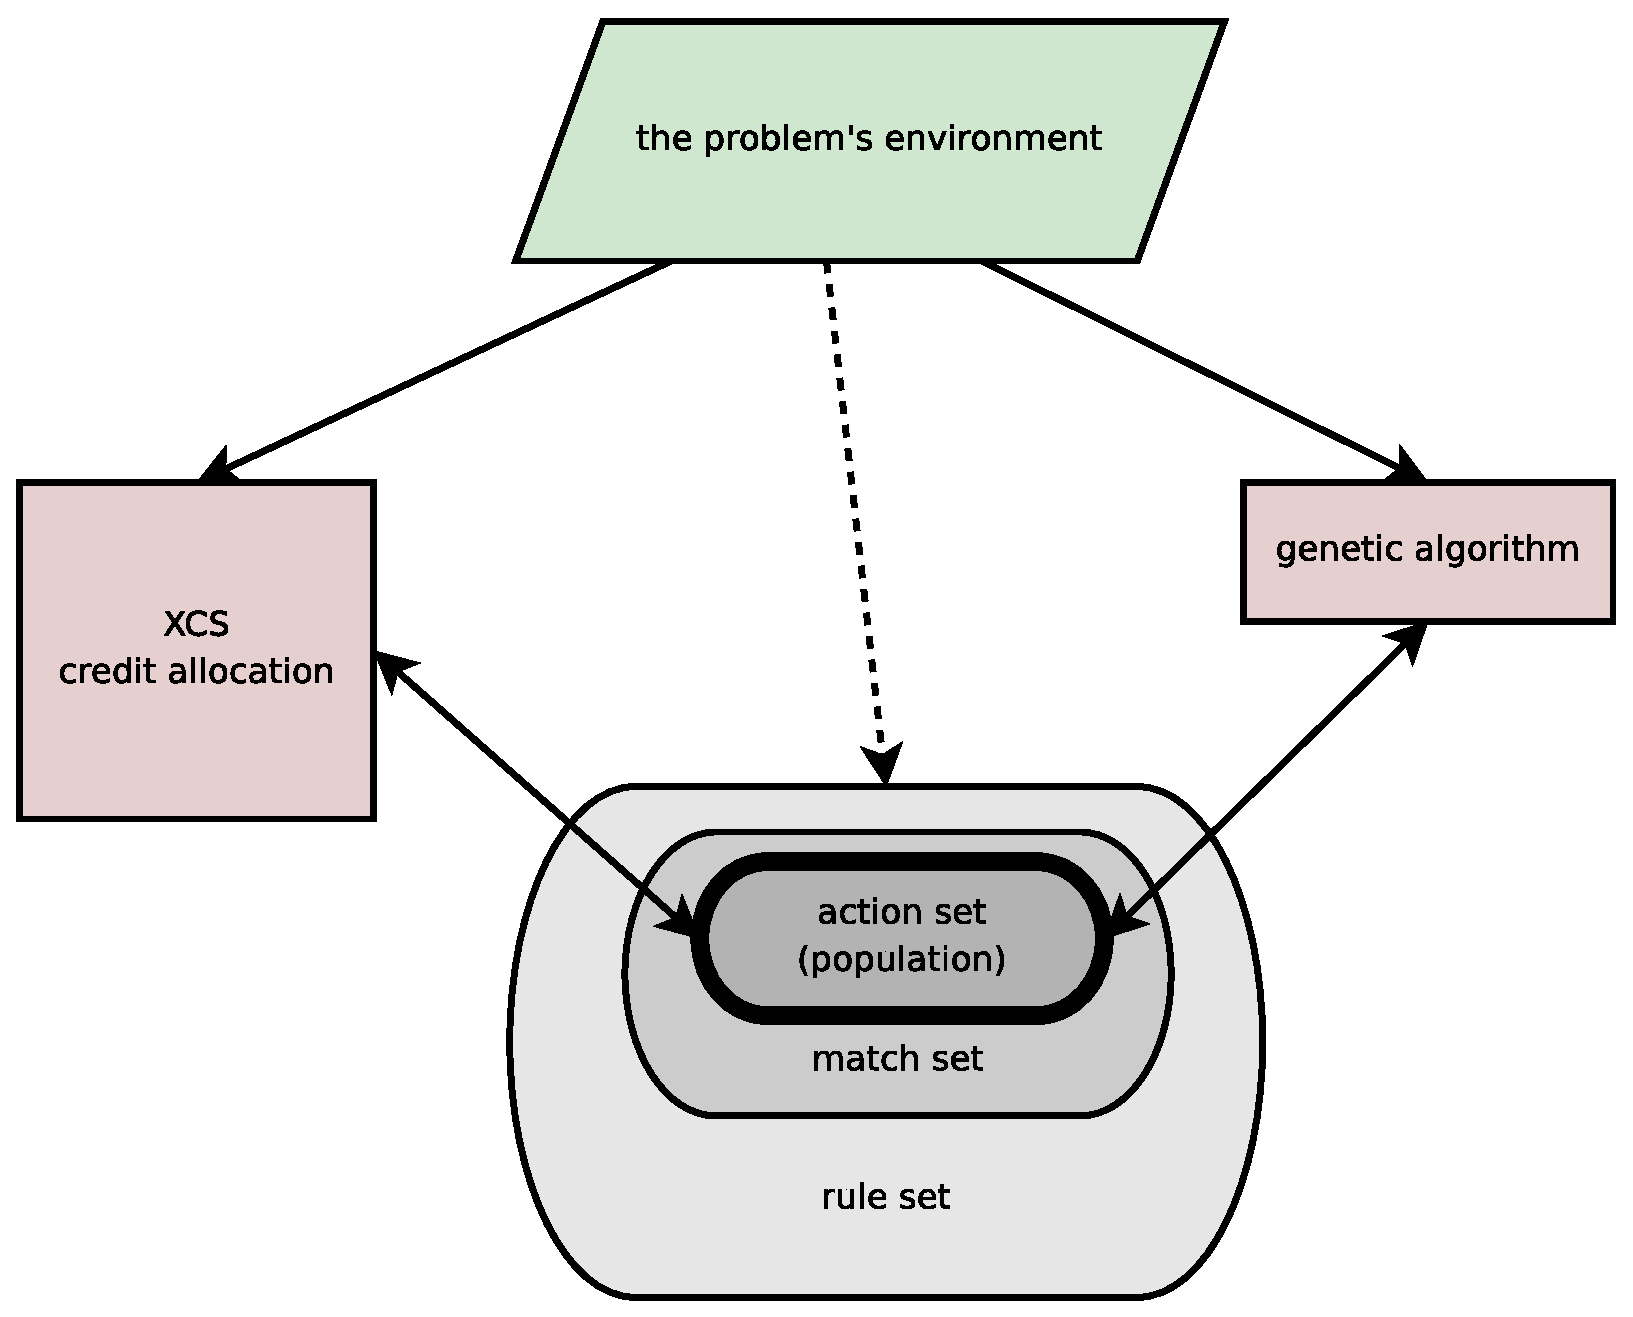
\includegraphics[width=4in]{xcs-basic-diagram.eps}
\caption{XCS's basic structure}
\label{fig:xcs}
\end{center}
\end{figure}

Each rule $r$ is now of the  more complex form
\begin{equation}
r = (c, a, p, \epsilon, F, exp, ts, as, n),
\end{equation}
where:
\begin{itemize}
\item
$c$ is the condition matched by the rule $r$, comprised of elements from some alphabet such as $\{0, 1, \#\}$,
where \# is the matching symbol, matching both 0 and 1.
\item
$a$ is the action that the rule $r$ recommends.
\item
$p$ is the predicted payoff.
\item
$\epsilon$ is an estimate of the prediction error.
\item
$F$ is the fitness used by the GA.
It is vital that the fitness used by the GA is a measure of the \emph{accuracy} of the rule,
and not a measure of the \emph{magnitude} of the rule, where the magnitude of a rule is how active that rule is in relation to the rest of the rules in the rule set, since a rule with greater magnitude but lower accuracy can be a detriment to the system.
For example, a rule that always matched every situation (all \#'s in the condition) but only accurately predicted 51\% of the situations would have high magnitude but low accuracy.
\item
$exp$ is the experience of the rule,
a count of the number of times since this classifier's creation that it has belonged to the action set.
\item
$ts$ is a time stamp of the last occurrence of a call to the GA in an action set that this classifier was a part of, as the generational number.
\item
$as$ is an estimate of the average action set size this classifier has belonged to.
\item
$n$ is the numerosity of this macro-classifier.
This is how many traditional micro-classifiers this macro-classifier represents.
Groups of entirely identical normal classifiers (the micro-classifiers) are subsumed into macro-classifiers instead of being allowed to exist separately within the rule set; this serves solely as a computational time-saver.
Therefore the only difference between a normal classifier (a micro-classifier) and a macro-classifier is the presence of the numerosity, which is a count of how many micro-classifiers that specific macro-classifier represents.
\end{itemize}


\subsubsection{XCSR}
\index{XCSR}
Wilson extended his concept of XCS with XCSR in \cite{WilsonXCSR}.
Classifier systems had typically taken strings from some small alphabet, often binary, as input until then
even though many real-world problems have input from the environment of the form $\mathbb{R}^n$ for some order $n \in \mathbb{Z}, n>0$.
Wilson's XCSR allows XCS to operate on just such an input.
XCSR is identical to normal XCS with the exception of the input interface, the nature of the predicates, the mutation operator, and the details of covering.
The basic structure of an XCSR rule is graphically illustrated in Figure~\ref{fig:xcsr-rule}.

Originally the predicates in XCSR were intervals of the form
\begin{equation}
interval_i = \{center_i,spread_i\},
\end{equation}
such that an environmental input $x_i$ was matched by $interval_i$ if and only if
\begin{equation}
center_i-spread_i \le x_i \le center_i+spread_i,
\end{equation}
but this was discovered to induce a bias \cite{StoneBull:2003}, so the representation was eventually changed to be
\begin{equation}
interval_i = \{lower_i,upper_i\},
\end{equation}
where now $x_i$ is matched by $interval_i$ if and only if
\begin{equation}
lower_i \le x_i \le upper_i.
\end{equation}
We use the $\{lower,upper\}$ form in this work.

\begin{figure}
\begin{center}
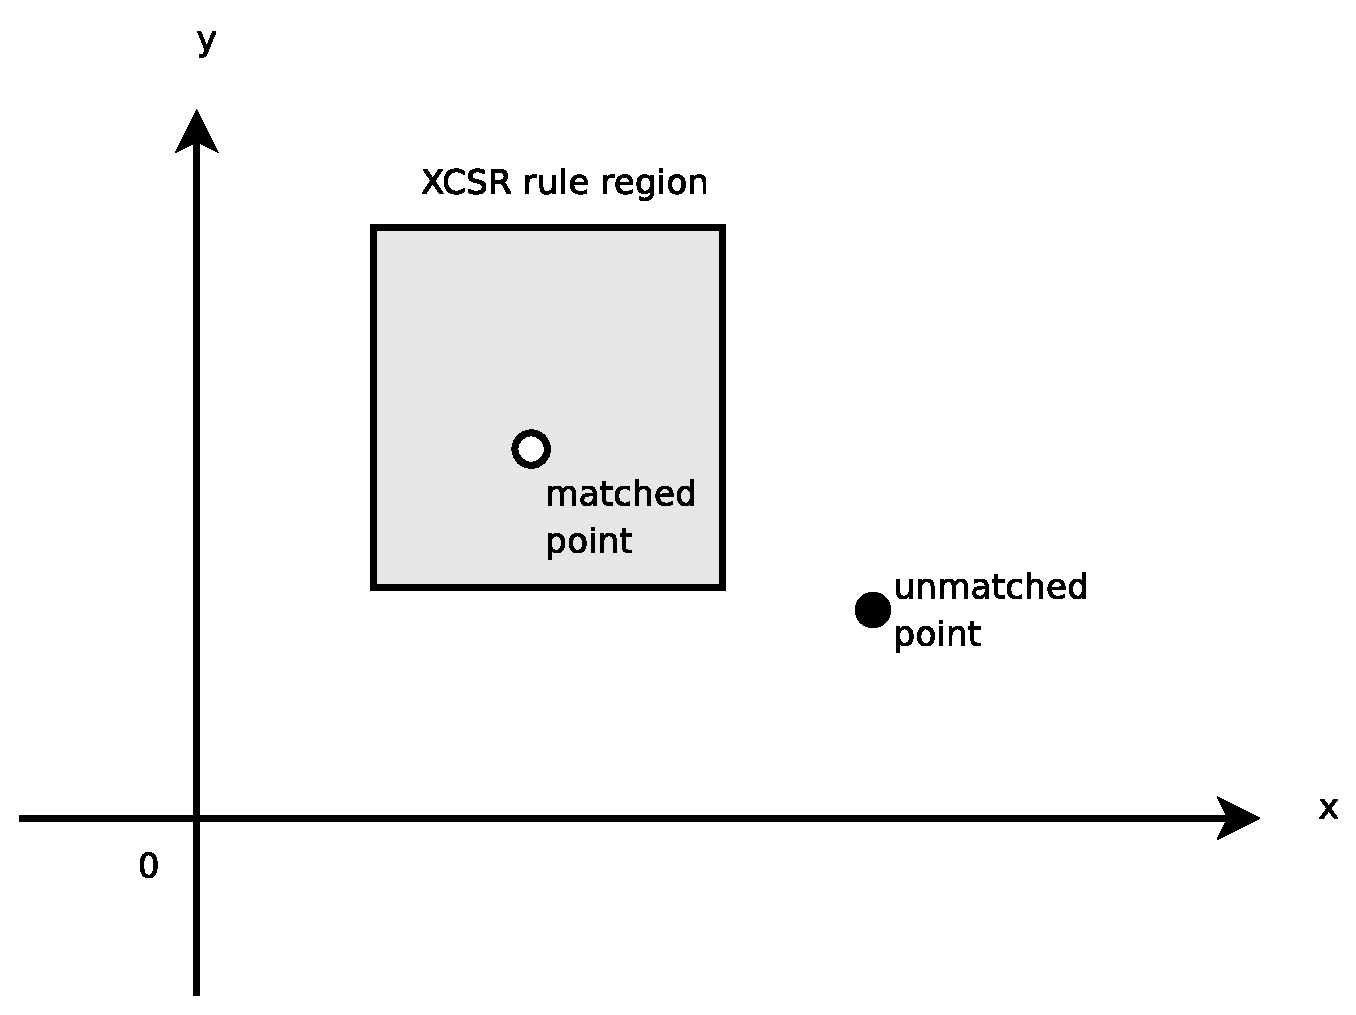
\includegraphics[width=4in]{xcsr-interval.eps}
\caption{XCSR's interval rules}
\label{fig:xcsr-rule}
\end{center}
\end{figure}

\newpage
Crossover is simple two-point crossover, but on the sequence
\begin{equation}
\{center_0,spread_0, \ldots\}
\end{equation}
or
\begin{equation}
\{lower_0,upper_0, \ldots\}
\end{equation}
depending on the predicate type,
in both cases therefore allowing the crossover points to fall within a single allele.

In the original XCSR, mutation was performed by adding a small random quantity from the range $[-0.1,0.1]$ to each allele, and all problems were to have their input scaled to $[0,1]$.
The variation of XCSR used here is capable of scaling outside of $[0.0,1.0]$, so instead mutation is performed as the addition or subtraction of a small percentage of the overall range as seen so far.


